\documentclass[usenames,dvipsnames,tikz]{standalone}
\usetikzlibrary{shapes.geometric}
\usepackage{xcolor}
\colorlet{tBlue}{RoyalBlue!35!Cerulean}
\colorlet{tRed}{Red}
\usepackage{tikz}
\usepackage{standalone}
\begin{document}
	
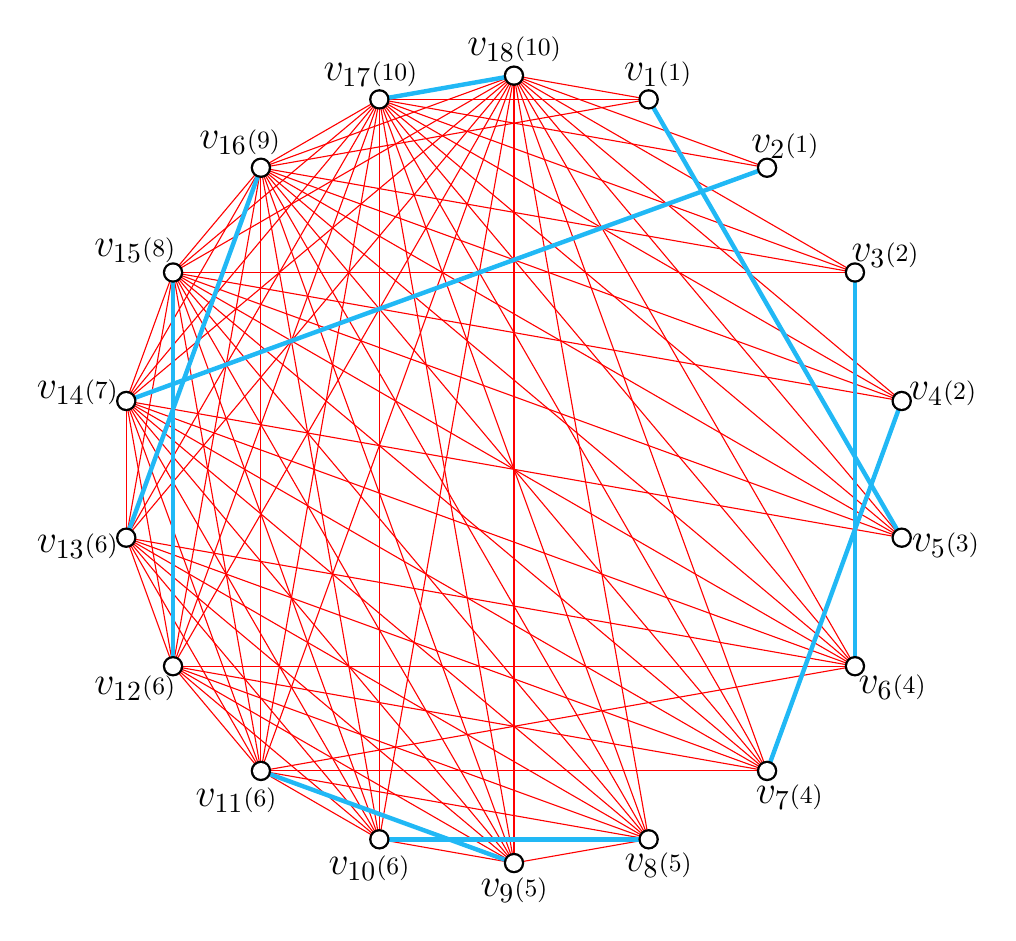
\begin{tikzpicture}
%Values of vertices:
% v1=1, v2=1, v3=2, v4=2, v5=3, v6=4, v7=4, v8=5, v9=5, v10=6, v11=6, v12=6, v13=6, v14=7, v15=8, v16=9, v17=10, v18=10 (v17/v18 universal vertices), \tau = 10.


\foreach \n/\value in {1/1, 2/1, 3/2, 4/2, 5/3, 6/4, 7/4, 8/5, 9/5, 10/6, 11/6, 12/6, 13/6, 14/7, 15/8, 16/9, 17/10, 18/10}
	\fill (90-\n*20:5cm) coordinate (v\n) circle [radius = 0.1];
	
\foreach \n/\value in {1/1, 17/10, 18/10}
	\fill (90-\n*20:5cm) coordinate (v\n) circle [radius = 0.1]
		++(90-\n*20:9.5pt) node {\Large{$v_{\n}$}\small{(\value)}};

\foreach \n/\value in {2/1, 8/5, 9/5}
	\fill (90-\n*20:5cm) coordinate (v\n) circle [radius = 0.1]
		++(90-\n*20:10pt) node {\Large{$v_{\n}$}\small{(\value)}};
		
\foreach \n/\value in {3/2, 7/4}
	\fill (90-\n*20:5cm) coordinate (v\n) circle [radius = 0.1]
		++(90-\n*20:12.5pt) node {\Large{$v_{\n}$}\small{(\value)}};		
		

\foreach \n/\value in {4/2}
	\fill (90-\n*20:5cm) coordinate (v\n) circle [radius = 0.1]
		++(90-\n*20:15pt) node {\Large{$v_{\n}$}\small{(\value)}};

\foreach \n/\value in {5/3, 12/6, 15/8}
	\fill (90-\n*20:5cm) coordinate (v\n) circle [radius = 0.1]
		++(90-\n*20:16pt) node {\Large{$v_{\n}$}\small{(\value)}};
	
\foreach \n/\value in {6/4}
	\fill (90-\n*20:5cm) coordinate (v\n) circle [radius = 0.1]
		++(90-\n*20:15.5pt) node {\Large{$v_{\n}$}\small{(\value)}};
		
\foreach \n/\value in {10/6}
	\fill (90-\n*20:5cm) coordinate (v\n) circle [radius = 0.1]
		++(90-\n*20:11pt) node {\Large{$v_{\n}$}\small{(\value)}};
		
\foreach \n/\value in {11/6}
	\fill (90-\n*20:5cm) coordinate (v\n) circle [radius = 0.1]
		++(90-\n*20:14pt) node {\Large{$v_{\n}$}\small{(\value)}};
		
\foreach \n/\value in {13/6, 14/7}
	\fill (90-\n*20:5cm) coordinate (v\n) circle [radius = 0.1]
		++(90-\n*20:18pt) node {\Large{$v_{\n}$}\small{(\value)}};	

\foreach \n/\value in {16/9}
	\fill (90-\n*20:5cm) coordinate (v\n) circle [radius = 0.1]
		++(90-\n*20:12pt) node {\Large{$v_{\n}$}\small{(\value)}};	
	
	
%Edges and vertices
\foreach \m/\n in {1/16, 1/17, 1/18, 2/17, 2/18, 3/15, 3/16, 3/17, 3/18, 4/15, 4/16, 4/17, 4/18, 5/14, 5/15, 5/16, 5/17, 5/18, 6/11, 6/12, 6/13, 6/14, 6/15, 6/16, 6/17, 6/18, 7/11, 7/12, 7/13, 7/14, 7/15, 7/16, 7/17, 7/18, 8/9, 8/11, 8/12, 8/13, 8/14, 8/15, 8/16, 8/17, 8/18, 9/10, 9/12, 9/13, 9/14, 9/15, 9/16, 9/17, 9/18, 10/11, 10/12, 10/13, 10/14, 10/15, 10/16, 10/17, 10/18, 11/12, 11/13, 11/14, 11/15, 11/16, 11/17, 11/18, 12/13, 12/14, 12/16, 12/17, 12/18, 13/14, 13/15, 13/17, 13/18, 14/15, 14/16, 14/17, 14/18,	15/16, 15/17, 15/18, 16/17, 16/18}
	\draw [tRed] (v\n) -- (v\m);
\foreach \m/\n in {1/5, 2/14, 3/6, 4/7, 8/10, 9/11, 12/15, 13/16, 17/18}
	\draw [ultra thick, tBlue] (v\n) -- (v\m);
\foreach \n in {1,...,18}
	\fill (90-\n*20:5cm) coordinate (v\n) circle [radius = 0.13];
\foreach \n in {1,...,18}
	\fill [white] (90-\n*20:5cm) coordinate (v\n) circle [radius = 0.1];

\end{tikzpicture}
	
\end{document}